\documentclass[aspectratio=169]{beamer}
\usepackage[utf8]{inputenc}
\usepackage[vietnamese]{babel}
\usepackage{graphicx}
\usepackage{hyperref}
\usepackage{booktabs}
\usepackage{multicol}
\usepackage{amsmath}
\usepackage{xcolor}

\usetheme{Madrid}
\usecolortheme{whale}

\title[Dự báo thời tiết với Học Sâu]{Dự báo thời tiết ngắn hạn cho nông nghiệp chính xác ở Jammu và Kashmir:\\Phương pháp tiếp cận Học Sâu}
\author[GV: Trần Thanh Thắng]{ThS. Trần Thanh Thắng}
\institute[Đông Á University]{Khoa Công nghệ thông tin\\Đại học Đông Á}
\date{\today}

\begin{document}

\begin{frame}
    \titlepage
\end{frame}

\begin{frame}{Nội dung trình bày}
    \tableofcontents
\end{frame}

\section{Giới thiệu \& Đặt vấn đề}

\begin{frame}{Tầm quan trọng của dự báo thời tiết trong nông nghiệp}
    \begin{itemize}
        \item Thời tiết là yếu tố then chốt quyết định năng suất và chất lượng cây trồng.
        \item Thay đổi khí hậu cực đoan làm gia tăng rủi ro đối với nông nghiệp, đòi hỏi sự can thiệp của nông nghiệp thông minh và chính xác.
        \item Lợi ích của dự báo thời tiết (WF) ngắn hạn:
        \begin{itemize}
            \item Hỗ trợ ra quyết định kịp thời về tưới tiêu, bón phân, thu hoạch.
            \item Giảm thiểu tổn thất do điều kiện thời tiết bất lợi.
            \item Tối ưu hóa việc sử dụng các nguồn tài nguyên nông nghiệp.
        \end{itemize}
    \end{itemize}
\end{frame}

\begin{frame}{Vai trò của AI/Học sâu trong dự báo thời tiết}
    \begin{itemize}
        \item \textbf{Mô hình truyền thống}: 
        \begin{itemize}
            \item Dự báo thời tiết bằng số (NWP) thường đòi hỏi tính toán lớn và siêu máy tính.
            \item Mô hình thống kê (như ARMA, ARIMA) gặp khó khăn khi mô hình hóa dữ liệu phi tuyến tính phức tạp.
        \end{itemize}
        \item \textbf{Phương pháp tiếp cận bằng Học Sâu (Deep Learning)}:
        \begin{itemize}
            \item Khả năng học các biểu diễn phi tuyến tính trực tiếp từ dữ liệu lớn.
            \item Xử lý tốt dữ liệu chuỗi thời gian thông qua các mô hình Mạng Nơ-ron Hồi quy (RNN), LSTM, GRU.
            \item Độc lập và ít tốn kém tài nguyên tính toán hơn so với NWP.
        \end{itemize}
    \end{itemize}
\end{frame}

\begin{frame}{Đóng góp chính của nghiên cứu}
    \begin{itemize}
        \item Cung cấp hệ thống dự báo thời tiết ngắn hạn sử dụng mô hình \textbf{RNN (Mạng Nơ-ron Hồi quy)} tinh gọn.
        \item Giảm thiểu gánh nặng về mặt kỹ thuật và chi phí (không cần tới siêu máy tính như các phương pháp truyền thống).
        \item Hệ thống có thể triển khai tại địa phương, đặc biệt thích hợp cho các khu vực bị ảnh hưởng mạnh bởi biến đổi khí hậu như Jammu và Kashmir.
        \item Hỗ trợ nông dân chuẩn bị tốt hơn trước những thay đổi đột ngột của thời tiết, từ đó tối ưu hóa quy trình trồng trọt.
    \end{itemize}
\end{frame}

\section{Cơ sở lý thuyết \& Công trình liên quan}

\begin{frame}{Tổng quan các công trình liên quan}
    \begin{itemize}
        \item \textbf{Machine Learning (Học máy)}:
        \begin{itemize}
            \item Các thuật toán như RF (Random Forest), SVM (Support Vector Machine) và SVR được sử dụng rộng rãi để dự đoán cường độ lượng mưa và lũ lụt.
            \item Mô hình thống kê ARIMA truyền thống được dùng phân tích xu hướng nhiệt độ và lượng mưa.
        \end{itemize}
        \item \textbf{Deep Learning (Học Sâu)}:
        \begin{itemize}
            \item Mạng Nơ-ron Nhân tạo (ANN) và LSTM (Long Short-Term Memory) dần thay thế các mô hình truyền thống nhờ khả năng ghi nhớ dài hạn.
            \item Các nghiên cứu cho thấy mô hình RNN và LSTM có khả năng tái tạo chuỗi thời gian khí tượng chính xác, phục vụ từ dự báo lượng mưa đến mực nước hồ chứa.
        \end{itemize}
    \end{itemize}
\end{frame}

\begin{frame}{Giới thiệu Mạng Nơ-ron Hồi quy (RNN)}
    \begin{itemize}
        \item \textbf{Định nghĩa}: RNN là một loại Mạng nơ-ron nhân tạo được thiết kế đặc biệt để xử lý dữ liệu chuỗi (sequence data) và chuỗi thời gian (time-series).
        \item \textbf{Ưu điểm cốt lõi}:
        \begin{itemize}
            \item Khác với Feedforward Neural Networks, RNN có \textbf{\textit{bộ nhớ trong}} thông qua các vòng lặp phản hồi (feedback loops).
            \item Nó sử dụng trạng thái ẩn (hidden state) từ bước thời gian trước đó để làm đầu vào cho bước thời gian hiện tại.
        \end{itemize}
        \item Phù hợp hoàn hảo cho việc dự báo nhiệt độ, độ ẩm dựa trên dữ liệu khí tượng của các ngày trước đó.
    \end{itemize}
\end{frame}

\begin{frame}{Hoạt động của RNN}
    \begin{figure}[h!]
        \centering
        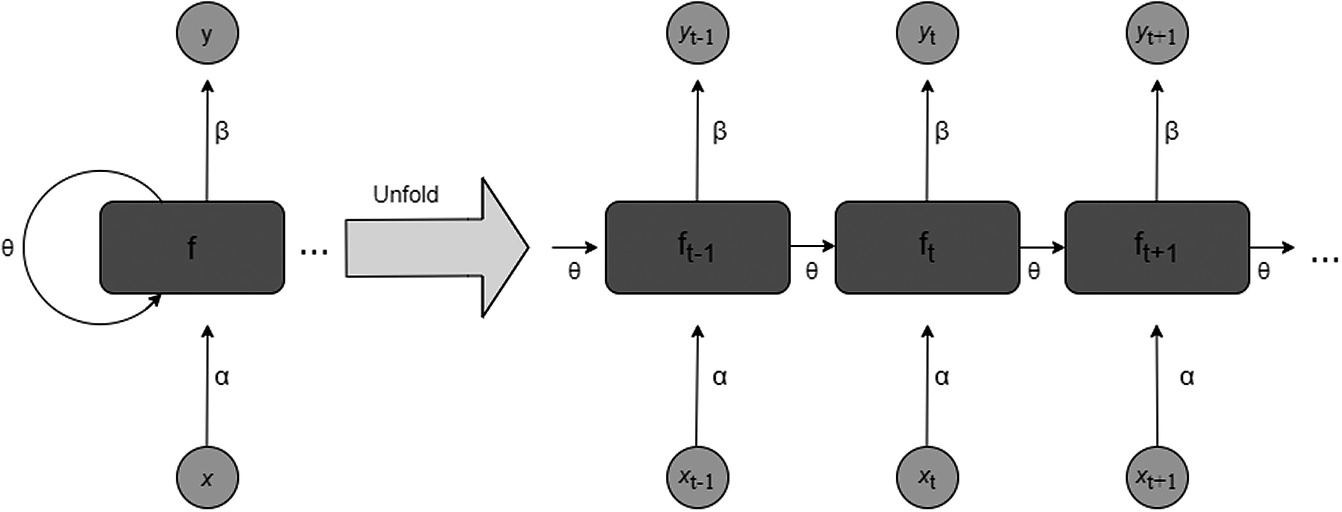
\includegraphics[width=0.95\textwidth,height=0.65\textheight,keepaspectratio]{images/chap14/img_4_0.png}
        \caption{Cơ chế hoạt động của Mạng nơ-ron hồi quy (RNN)}
    \end{figure}
\end{frame}

\begin{frame}{Thuật toán Lan truyền ngược theo thời gian (BPTT)}
    \begin{itemize}
        \item \textbf{BPTT (Backpropagation Through Time)} là phiên bản mở rộng của thuật toán Lan truyền ngược (Backpropagation) dành cho RNN.
        \item Quá trình:
        \begin{itemize}
            \item Tính toán mất mát (Loss) tại mỗi bước thời gian $t$.
            \item Truyền ngược lỗi (error) từ bước thời gian cuối cùng trở về các bước thời gian trước đó để cập nhật trọng số.
        \end{itemize}
        \item Giúp RNN học được các phụ thuộc thời gian (temporal dependencies) trong dữ liệu khí hậu.
        \item Hạn chế: Dễ gặp vấn đề triệt tiêu đạo hàm (vanishing gradient) khi chuỗi thời gian quá dài.
    \end{itemize}
\end{frame}

\section{Thử nghiệm \& Xây dựng mô hình}

\begin{frame}{Quy trình Lập mô hình}
    \begin{figure}[h!]
        \centering
        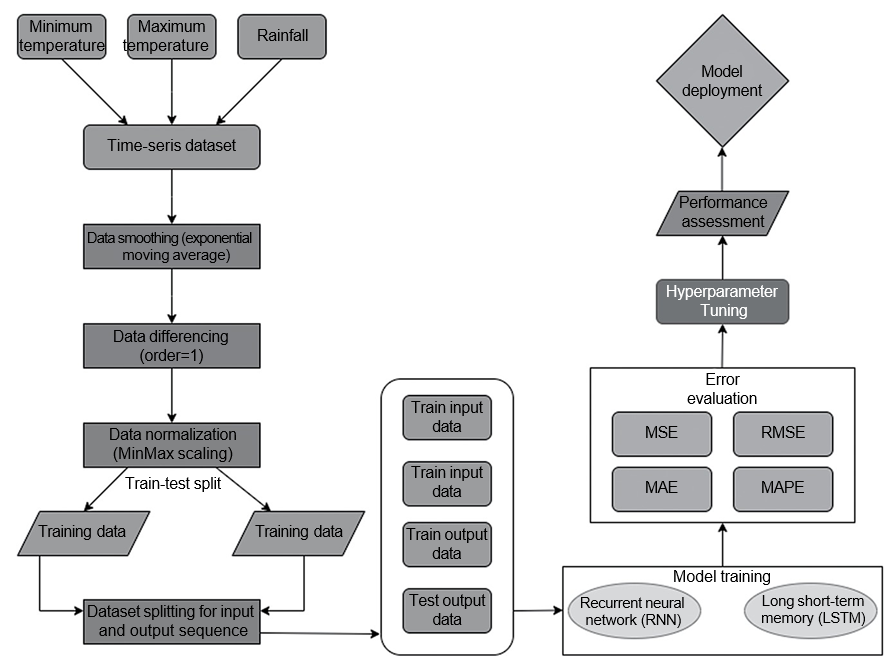
\includegraphics[width=0.95\textwidth,height=0.65\textheight,keepaspectratio]{images/chap14/img_7_0.png}
        \caption{Quy trình thu thập, xử lý và xây dựng mô hình Học Sâu}
    \end{figure}
\end{frame}

\begin{frame}{Thu thập và Tiền xử lý Dữ liệu}
    \begin{itemize}
        \item \textbf{Bộ dữ liệu}:
        \begin{itemize}
            \item Thu thập từ 3 trạm quan trắc tại Jammu và Kashmir: Jammu (Cận nhiệt đới), Srinagar (Ôn đới), Leh (Lạnh và Khô).
            \item Giai đoạn: 2010 đến 2022. Các thông số: Nhiệt độ trung bình ($T_{avg}$), Nhiệt độ tối đa ($T_{max}$), Nhiệt độ tối thiểu ($T_{min}$).
        \end{itemize}
        \item \textbf{Tiền xử lý}:
        \begin{itemize}
            \item \textit{Trích xuất xu hướng}: Áp dụng EMA (Exponential Moving Average) để làm mịn dữ liệu.
            \item \textit{Tính dừng}: Sử dụng sai phân bậc 1 (First-order differencing).
            \item \textit{Chuẩn hóa}: MinMax Scaler để quy đổi dữ liệu về khoảng [0, 1].
        \end{itemize}
    \end{itemize}
\end{frame}

\begin{frame}{Cấu hình và Huấn luyện}
    \begin{itemize}
        \item \textbf{Cấu trúc mô hình}: Sử dụng Keras/TensorFlow.
        \begin{itemize}
            \item Lớp ẩn chứa 16-32 nơ-ron RNN. Lớp đầu ra (Dense).
            \item Các cấu hình kiểm thử: \textbf{SISO} (Single Input Single Output) và \textbf{MIMO} (Multiple Input Multiple Output).
        \end{itemize}
        \item \textbf{Tối ưu siêu tham số}: Dùng \textit{GridSearchCV} cho epochs (50, 100), kích thước batch (32, 64) và các thuật toán tối ưu (Adam, RMSprop).
        \item \textbf{Cửa sổ trượt (Sliding Window)}: Sử dụng $K$ ngày trong quá khứ để dự đoán $T$ ngày tiếp theo.
    \end{itemize}
\end{frame}

\begin{frame}{Các chỉ số đánh giá}
    \begin{itemize}
        \item Để đo lường mức độ sai số giữa giá trị dự báo và giá trị thực tế, mô hình sử dụng các chỉ số:
        \begin{itemize}
            \item \textbf{MAE (Mean Absolute Error)}: Trung bình sai số tuyệt đối.
            \item \textbf{MSE (Mean Squared Error)}: Trung bình bình phương sai số.
            \item \textbf{RMSE (Root Mean Squared Error)}: Căn bậc hai của MSE.
            \item \textbf{MAPE (Mean Absolute Percentage Error)}: Phần trăm sai số trung bình tuyệt đối.
        \end{itemize}
        \item Giá trị các chỉ số này càng nhỏ, mô hình dự báo càng chính xác.
    \end{itemize}
\end{frame}

\section{Kết quả \& Kết luận}

\begin{frame}{Kết quả Huấn luyện (SISO vs MIMO)}
    \begin{itemize}
        \item \textbf{Kết quả chính}: Phương pháp SISO mang lại độ chính xác cao hơn MIMO trên toàn bộ 3 trạm quan trắc (Jammu, Srinagar, Leh).
        \item \textbf{Nguyên nhân}:
        \begin{itemize}
            \item Các thông số nhiệt độ ($T_{max}$, $T_{min}$, $T_{avg}$) có sự phụ thuộc lẫn nhau yếu trong khu vực.
            \item Mô hình hóa thành các biến độc lập đơn biến (SISO) giúp mạng RNN dễ dàng bắt được quy luật của từng biến mà không bị nhiễu bởi các biến khác.
        \end{itemize}
        \item Mô hình tối ưu được xác định sử dụng bộ tối ưu \textbf{Adam}, với \textbf{batch size=32} và \textbf{epochs=50}.
    \end{itemize}
\end{frame}

\begin{frame}{Bảng tổng hợp kết quả (Ví dụ với $T_{max}$)}
    \begin{itemize}
        \item Mô hình RNN cấu hình SISO cho thấy sai số cực kỳ nhỏ:
        \begin{itemize}
            \item Tại trạm \textbf{Srinagar}: MSE $\approx 0.0003$, MAE $\approx 0.0123$.
            \item Tại trạm \textbf{Jammu}: MSE $\approx 0.0001$, MAE $\approx 0.0075$.
            \item Tại trạm \textbf{Leh}: MSE $\approx 0.0002$, MAE $\approx 0.0076$.
        \end{itemize}
        \item Dữ liệu cho thấy mô hình hoàn toàn có khả năng tái tạo chuỗi nhiệt độ khí tượng chính xác cho các khoảng dự báo ngắn (1-10 ngày).
    \end{itemize}
\end{frame}

\begin{frame}{Kết luận}
    \begin{itemize}
        \item Mạng Nơ-ron Hồi quy (RNN) đã chứng minh được tính hiệu quả cao trong bài toán dự báo thời tiết ngắn hạn thông qua việc nắm bắt sự phụ thuộc phi tuyến.
        \item Việc tiếp cận cấu hình SISO là hướng đi chính xác cho các bộ dữ liệu khí tượng có tính độc lập cao.
        \item Mô hình này gọn nhẹ, yêu cầu năng lực tính toán thấp, do đó hoàn toàn \textbf{có thể triển khai trực tiếp cho bà con nông dân địa phương} sử dụng trên máy tính thông thường hoặc thiết bị thông minh.
    \end{itemize}
\end{frame}

\begin{frame}{Định hướng tương lai}
    \begin{itemize}
        \item \textbf{Mở rộng dữ liệu}: Đưa thêm các tham số quan trọng như độ ẩm, lượng mưa, tốc độ gió, và lượng mây vào mô hình.
        \item \textbf{Khám phá MIMO}: Tối ưu hóa kiến trúc mạng để phương pháp MIMO có thể khai thác sự tương quan đa biến (nếu có) khi bổ sung thêm các yếu tố thời tiết mới.
        \item \textbf{Cải tiến mô hình}: Thử nghiệm các cấu trúc Học sâu tiên tiến hơn (như LSTM, GRU, Transformers) để giải quyết vấn đề quên dài hạn của RNN cơ bản.
    \end{itemize}
\end{frame}

\begin{frame}
    \centering
    \Huge \textbf{Hỏi \& Đáp} \\
    \vspace{1cm}
    \large Xin trân trọng cảm ơn!
\end{frame}

\end{document}
